%!TEX root = ../clcxsj.tex

\chapter{高斯投影程序设计}

高斯投影是为解决球面与平面之间的坐标映射问题,即大地坐标(B,
L)与高斯平面直角坐标$(x,y)$之间的相互换算,以及不同带之间的高斯坐标
的换算问题。

高斯投影是我国1:50万以及更大比例尺地形图的数学基础,我国自1953年开始就采用,也是世界不少国家的地形图基础。
高斯投影在低纬度地区变形较大,在纬度30以下投影带的边缘部分变形值超过 1/1000 。
对低纬度地区地形图不是很适宜,对高纬度地区的地形图较好。

通用横墨卡托(Universal Transverse Mercator)简称为 UTM 投影,是横割圆柱投影,投影方法与高斯投影基本相同。
但每带中央子午线的长度比为 0.9996。
对中纬度地区与低纬度地区来讲,UTM投影优于高斯-克吕格投影。
UTM投影是目前美国、德国等60多个国家的国家基本地形图的数学基础。

本章将运用$C\#$编程语言编写一个通用的高斯投影程序,用于1954北京坐标系、1980西安坐标系、
WGS84坐标系以及CGCS2000大地坐标系或自定义参考椭球的高斯投影正反算与换带计算。


\section{高斯投影的数学模型}

为了编制正确而且高效的高斯投影与换带程序,我们首先需要分析高斯投影的数学模型,也就是我们
常说的算法。

本章所引用的公式来自:
孔祥元,郭际明,刘宗泉.大地测量学基础-2版.武汉:武汉大学出版社,2010.5,
以下将这本书简称为大地测量学基础或大地测量学。

\subsection{椭球基础}
投影是基于参考椭球进行的,所以首先需要分析参考椭球的计算。

高斯投影是在椭球的几何参数(长半轴a、短半轴b、扁率$\alpha$)确定的条件下,根据
给定的数学模型来进行计算的,我们首先分析这些计算公式与数学模型。

\begin{enumerate}

\item 基本公式

\begin{enumerate}
\item 扁率:
$$\alpha=\frac{a-b}{a}$$

\item 第一偏心率:
$$e=\sqrt{\frac{a^2-b^2}{a^2}}$$

\item 第二偏心率:
$$e'=\sqrt{\frac{a^{2}-b^{2}}{b^{2}}}$$

\item 子午圈曲率半径:
$$M=\frac{a(1-e^2)}{(1-e^2\sin ^2 B)^{\frac{3}{2}}}$$

\item 卯酉圈曲率半径:
$$N=\frac{a}{\sqrt{1-e^2\sin^2 B}}$$

\item 辅助符号:
$$t=\tan B\qquad\eta=e'\cos B$$
\end{enumerate}

\item 椭球面梯形图幅面积计算

$$P = \frac{b^2}{2}(L_2 - L_1) \left | \frac{\sin B}{1-e^2\sin^2 B} 
+ \frac{1}{2e}\ln \frac{1+e\sin B}{1-e\sin B}\right |_{B1} ^{B2} $$
公式引用自《大地测量学基础》第121页(4-140)。

$$P=b^2(L_2 - L_1) \left | sinB + \frac{2}{3}e^2 \sin ^3 B 
+ \frac{3}{5}e^4 \sin^5 B + \frac{4}{7}e^6 \sin ^7 B \right | _{B_1} ^{B_2}$$

公式引用自《大地测量学基础》第121页(4-142),该公式为(4-140)的展开式。

\item 子午线弧长
\begin{equation}
\label{eq:xx}
X=a_0 B - \frac{a_2}{2}\sin 2B + \frac{a_4}{4}\sin 4B
- \frac{a_6}{6} \sin 6B  + \frac{a_8}{8}\sin 8B
\end{equation}

式中:
\begin{equation}
\label{eq:xxaa}
\left  . \begin{aligned}
a_0 &= m_0 + \frac{m_2}{2} + \frac{3}{8}m_4 + \frac{5}{16}m_6 + \frac{35}{128}m_8  \\
a_2 &= \frac{m_2}{2} + \frac{m_4}{2} + \frac{15}{32}m_6 + \frac{7}{16}m_8  \\
a_4 &= \frac{m_4}{8} + \frac{3}{16}m_6 + \frac{7}{32}m_8  \\
a_6 &= \frac{m_6}{32} + \frac{m_8}{16}  \\
a_8 &= \frac{m_8}{128}
\end{aligned} \right \}
\end{equation}

式中$m_0, m_2, m_4, m_6, m_8$的值为:

\begin{equation}
\label{eq:xxmm}
\left . 
\begin{aligned}
m_0 &= a(1-e^2) \\
m_2 &= \frac{3}{2}e^2 m_0  \\
m_4 &= \frac{5}{4}e^2 m_2  = \frac{15}{8} e^4 m_0 \\
m_6 &= \frac{7}{6}e^2 m_4   = \frac{35}{16} e^6 m_0 \\
m_8 &= \frac{9}{8}e^2 m_6 = \frac{315}{128} e^8 m_0
\end{aligned} 
\right \}
\end{equation}

以上公式引用自《大地测量学基础》第115页(4-101)、(4-100)与(4-72).

将公式 \ref{eq:xxmm} 代入公式  \ref{eq:xxaa}可得到如下公式:

 \begin{equation}
\label{eq:xxaamm}
\left  . \begin{aligned}
a_0 &=(1 + \frac{3}{4} e^2 + \frac{45}{64} e^4 + \frac{175}{256} e^6 + \frac{11025}{16384} e^8) m_0  \\
a_2 &=(\frac{3}{4} e^2 + \frac{15}{16} e^4 + \frac{525}{512} e^6 + \frac{2205}{2048} e^8) m_0  \\
a_4 &=(\frac{15}{64} e^4 + \frac{105}{256} e^6 + \frac{2205}{4096} e^8) m_0  \\
a_6 &=(\frac{35}{512} e^6 + \frac{315}{2048} e^8) m_0  \\
a_8 &= \frac{315}{16384} e^8 m_0
\end{aligned} \right \}
\end{equation}

若令:
\begin{equation}
\label{eq:xxAAA}
\left  . \begin{aligned}
A_0 &=a_0 = (1 + \frac{3}{4} e^2 + \frac{45}{64} e^4 + \frac{175}{256} e^6 + \frac{11025}{16384} e^8) m_0  \\
A_2 &=-\frac{a2}{2} =-\frac{1}{2}  (\frac{3}{4} e^2 + \frac{15}{16} e^4 + \frac{525}{512} e^6 + \frac{2205}{2048} e^8) m_0  \\
A_4 &=\frac{a_4}{4}=\frac{1}{4} (\frac{15}{64} e^4 + \frac{105}{256} e^6 + \frac{2205}{4096} e^8) m_0  \\
A_6 &=-\frac{a_6}{6}=-\frac{1}{6} (\frac{35}{512} e^6 + \frac{315}{2048} e^8) m_0  \\
A_8 &= \frac{a_8}{8}=\frac{1}{8} \times \frac{315}{16384} e^8 m_0
\end{aligned} \right \}
\end{equation}

则子午线弧长公式 \ref{eq:xx}可以演变为如下公式:
\begin{equation}
\label{eq:AAAxxAAA}
X= A_0 B + A_2 \sin 2B + A_4 \sin 4B + A_6 \sin 6B  + A_8 \sin 8B
\end{equation}

公式 \ref{eq:AAAxxAAA} 将作为我们进行程序设计时进行子午线弧长与底点纬度计算的基本公式。

由公式 \ref{eq:xxAAA}看出,其值只与椭球的定义有关,一旦椭球的参数确定,这些值也就被确定。

% 或用很多书上都引用的公式:

% \begin{equation}
% \label{eq:CX}
% X=c[\beta_0 B + (\beta_2 \cos B + \beta_4 \cos^3 B + \beta_6 \cos^5 B + \beta_8 \cos^7 B) \sin B] 
% \end{equation}

% 式中 c 为极曲率半径,其值为: $c= a^2 / b$,
% $\beta_0, \beta_2, \beta_4, \beta_6, \beta_8$的值为:

% \begin{equation}
% \label{eq:CXC}
% \left .
% \begin{aligned}
% \beta_0 &= 1 - \frac{3}{4}e'^2 + \frac{45}{64}e'^4 - \frac{175}{256}e'^6 + \frac{11025}{16384}e'^8  \\
% \beta_2 &= \beta_0 -1  \\
% \beta_4 &= \frac{15}{32}e'^4 - \frac{175}{384}e'^6 + \frac{3675}{8192}e'^8   \\
% \beta_6 &= -\frac{35}{96}e'^6 + \frac{735}{2048}e'^8   \\
% \beta_8 &= \frac{315}{1024}e'^8
% \end{aligned} 
% \right \}
% \end{equation}

% 公式引用自《大地测量学基础》第115页(4-107)、与(4-108)。

% 可对公式\ref{eq:CXC}做进一步演化,令:
% \begin{equation}
% 	\label{eq:CXCC}
% 	\left .
% 	\begin{aligned}
% 		C_0 &= c \beta_0 = c(1 - \frac{3}{4}e'^2 + \frac{45}{64}e'^4 - \frac{175}{256}e'^6 + \frac{11025}{16384}e'^8) \\
% 		C_2 &= c \beta_2 = c(\beta_0 -1)                                                                              \\
% 		C_4 &= c \beta_4 = c(\frac{15}{32}e'^4 - \frac{175}{384}e'^6 + \frac{3675}{8192}e'^8)                         \\
% 		C_6 &= c \beta_6 = c(-\frac{35}{96}e'^6 + \frac{735}{2048}e'^8)                                               \\
% 		C_8 &= c \beta_8 = c(\frac{315}{1024}e'^8)
% 	\end{aligned}
% 	\right \}
% \end{equation}

% 则子午线弧长公式\ref{eq:CX}可演化为:

% \begin{equation}
% 	\label{eq:CXX}
% 	X=C_0 B + (C_2 \cos^2 B + C_4 \cos^4 B + C_6 \cos^6 B + C_8 \cos^8 B) \tan B
% \end{equation}

\subsection{高斯投影正算}

高斯投影正算就是将球面上一点的大地坐标 $(B, L)$ 投影为高斯平面直角坐标 $(x, y)$。

\item 高斯投影正算
\begin{equation}
\left .
\begin{aligned}
x&=X+\frac{l^2 N}{2}sinBcosB +\frac{l^4 N}{24}sinBcos^3B(5-t^2 +9\eta^2+4\eta^4) \\
  &+\frac{N}{720}sinBcos^5 B(61-58t^2 +t^4)l^6  \\
y&=l N cosB+\frac{l^3 N}{6}cos^3 B(1-t^2 +\eta^2 ) \\
        &+\frac{l^5 N}{120}cos^5 B (5-18t^2+t^4 +14\eta^2 -58\eta^2t^2)
\end{aligned}
 \right \}
\end{equation}

公式引用自《大地测量学基础》第169页(4-367)。

\item 高斯投影反算

\begin{equation}
\left  .
\begin{aligned}
B&=B_f - \frac{t_f}{2M_f N_f }y^2 +\frac{t_f}{24 M_f N_f ^3}
(5 + 3t_f ^2  + \eta_f ^2 - 9\eta_f ^2 t_f^2)y^4 \\
 &- \frac{t_f}{720 M_f N_f ^5}(61 + 90t_f ^2 + 45t_f ^4)y^6 \\
l&=\frac{1}{N_f cosB_f}y - \frac{1}{6N_f ^3 cosB_f}(1 + 2t_f ^2 + \eta_f ^2)y^3  \\
 &+ \frac{1}{120N_f ^5 cosB_f}(5 + 28t_f ^2 + 24t_f ^4 + 6\eta_f ^2 +8\eta_f ^2 t_f ^2)y^5
\end{aligned} 
\right \}
\end{equation}

公式引用自《大地测量学基础》第171页(4-383)。


\item 平面子午线收敛角计算

利用$(B, l)$计算公式如下:
$$\gamma = l \cdot \sin B  + \frac{l^3}{3} \sin B \cos ^2 B \cdot (1 + 3 \eta^2 + 2 \eta^4)
+ \frac{ l^5}{15}\sin B \cos ^4 B \cdot (2 - t^2)$$

公式引用自《大地测量学基础》第181页(4-408)。

利用$(x, y)$计算公式如下:

$$\gamma = \frac{1}{N_f}t_f y - \frac{1+t_f ^2 - \eta_f ^2}{3N_f ^3}t_f y^3
+ \frac{2+5t_f^2+3t_f^4}{15N_f ^5}t_fy^5$$

公式引用自《大地测量学基础》第182页(4-410)。

\item 长度比计算

利用$(B, l)$计算公式如下:
$$m=1+\frac{l^2}{2} \cos ^2 B(1+\eta^2) + \frac{l^4}{24}\cos ^4 B(5-4t^2)$$

公式引用自《大地测量学基础》第189页(4-447)。

利用$(x, y)$计算公式如下:

$$m=1+\frac{y^2}{2R^2} + \frac{y^4}{24R^4}$$

式中$R=\sqrt{MN}$,公式引用自《大地测量学基础》第189页(4-451)。

\end{enumerate}

\section{程序功能分析与设计}

\subsection{高斯投影的主要内容}
\begin{enumerate}
    \item 坐标正算:将点的大地坐标转换成高斯投影平面直角坐标。
    \item 坐标反算:将点的高斯投影平面直角坐标转换成大地坐标。
    \item 换带计算:将某带的点的高斯投影平面直角坐标转换成邻带或某中央
    子午线经度的高斯投影平面直角坐标。
    \item 其他计算:计算子午线收敛角、长度比等。
\end{enumerate}

\subsection{参考椭球类的设计}

分析以上各个计算公式发现,如果椭球长半轴与扁率确定,参考椭球的第一偏心率$e$、
第二偏心率$e'$,子午线弧长计算的辅助计算参数$(m_0, m_2, m_4, m_6, m_8)$与
$(a_0, a_2, a_4, a_6, a_8)$也就确定了,其中的$(m_0, m_2, m_4, m_6, m_8)$
作为计算$(a_0, a_2, a_4, a_6, a_8)$的值使用过一次。也就是说这些参数对于某一种确定的
参考椭球是常数。而$(M,N,t,\eta)$则是纬度$B$的函数。

我们新建一 WPF 项目,命名为GaussProj,程序中我们将应用WPF技术编写图形界面。

在高斯投影中由于要处理角度与点等数据,我们可将前面的角度处理函数DMS2RAD、RAD2DMS
与SPoint点类拷贝到当前项目中来,也可以将其打包成一 Class Library(.NET Framework)
即类库文件引用到当前项目中,在当前项目中尽量不修改前面的各个功能代码。

基于上一小节的分析,我们新建一椭球类$(Spheroid)$,在其中我们定义以上与椭球类型
相关的元素。代码如下所示:

\begin{lstlisting}[language=C]
namespace GaussProj
{
    /// <summary>
    /// 参考椭球
    /// </summary>
    public class Spheroid
    {
        /// <summary>
        /// 长半轴
        /// </summary>
        public double a { get; set; }

        /// <summary>
        /// 短半轴
        /// </summary>
        public double b { get; set; }

        /// <summary>
        /// 扁率分母
        /// </summary>
        public double f { get; set; }  //(a-b)/a = 1/f

        /// <summary>
        /// 第一偏心率的平方
        /// </summary>
        public double e2 { get; set; }

         /// <summary>
        /// 第二偏心率的平方
        /// </summary>
        public double eT2 { get; set; }

        //计算子午线弧长时的各个系数项
        private double a0;
        private double a2;
        private double a4;
        private double a6;
        private double a8;
    }
}
\end{lstlisting}

在各项计算中,第一偏心率与第二偏心率的直接使用较少,其平方值用的较多,因此在
Spheroid类我们直接用其平方值。

 在Spheroid类中我们可以如下直接定义构造函数用于初始化其各个字段(Field):
  \begin{lstlisting}[language=C]
/// <summary>
/// 构造函数
/// </summary>
private Spheroid(double semimajor_axis, double inverse_flattening)
{
    this.a = semimajor;
    this.f =  inverse_flattening;
    ...................................................
}
\end{lstlisting}

但这样我们可能无法为已知的一些参考椭球直接提供参数,所以我们将构造函数定义
为 private,让用户无法通过new直接创建实例化对象。我们设计类的静态函数
Create**** 来创建类Spheroid的实例化对象,其代码如下:

 \begin{lstlisting}[language=C]
/// <summary>
/// 构造函数
/// </summary>
private Spheroid(){}

/// <summary>
/// 初始化椭球参数的内部函数
/// </summary>
private void Init(double semimajor_axis, double inverse_flattening)
{
    this.a = semimajor_axis; this.f = inverse_flattening;
    b = a * (1 - 1 / f);

    e2 = 1 - b / a * b / a;
    eT2 = a / b * a / b - 1;

    double m0 = a * (1 - e2);
    double m2 = 3.0 / 2.0 * e2 * m0;
    double m4 = 5.0 / 4.0 * e2 * m2;
    double m6 = 7.0 / 6.0 * e2 * m4;
    double m8 = 9.0 / 8.0 * e2 * m6;

    a0 = m0 + m2 / 2.0 + 3.0 / 8.0 * m4 + 5.0 / 16.0 * m6
                  + 35.0 / 128.0 * m8;
    a2 = m2 / 2.0 + m4 / 2.0 + 15.0 / 32.0 * m6 + 7.0 / 16.0 * m8;
    a4 = m4 / 8.0 + 3.0 / 16.0 * m6 + 7.0 / 32.0 * m8;
    a6 = m6 / 32.0 + m8 / 16.0;
    a8 = m8 / 128.0;
}

public static Spheroid CreateBeiJing1954()
{
    Spheroid spheroid = new Spheroid();
    spheroid.Init(6378245, 298.3);
    return spheroid;
}

public static Spheroid CreateXian1980()
{
    Spheroid spheroid = new Spheroid();
    spheroid.Init(6378140, 298.257);
    return spheroid;
}

public static Spheroid CreateWGS1984()
{
    Spheroid spheroid = new Spheroid();
    spheroid.Init(6378137, 298.257223563);
    return spheroid;
}

public static Spheroid CreateCGCS2000()
{
    Spheroid spheroid = new Spheroid();
    spheroid.Init(6378137, 298.257222101);
    return spheroid;
}

public static Spheroid CreateCoordinateSystem(double semimajor_axis,
      double inverse_flattening)
{
    Spheroid spheroid = new Spheroid();
    spheroid.Init(semimajor_axis, inverse_flattening);
    return spheroid;
}
\end{lstlisting}

这种将构造函数设为private,通过静态函数来创建实例化对象的技术在软件设计中
会经常用到。同时在设计类的方法时,应注意访问权限的设置,如上面代码中Init函数,
在类中用于初始化椭球的各项几何参数,并不需要在类外来调用它,所以我们将其设置为
private权限。

\subsection{高斯投影正算功能的实现}
有了类Spheroid的设计,我们先来完成高斯投影正算功能。
为了避免在计算中频繁的进行度分秒与弧度之间的转换问题,
我们设定除了特别声明之外,在类Spheroid中所用的角度均为弧度。

我们将高斯投影正算的函数名称定义为 BLtoXY,其设计如下:

\begin{lstlisting}[language=C]
/// <summary>
/// 高斯投影正算
/// </summary>
/// <param name="B">纬度,单位:弧度</param>
/// <param name="L">经度,单位:弧度</param>
/// <param name="L0">中央子午线经度,单位:弧度</param>
/// <param name="x">高斯平面x坐标</param>
/// <param name="y">高斯平面y坐标</param>
public void BLtoXY(double B, double L, double L0,
    out double x, out double y)
{
    ......................................
}
\end{lstlisting}

由于函数的返回值为两个值x与y,无法以函数的返回值return的形式返回计算结果,
所以我们用函数参数 out 的形式将计算结果返回。

 由前面的高斯投影正算公式分析可知,高斯投影正算的计算较为简单,没有复杂的逻辑,
 先计算经差,然后计算子午线弧长后就可以直接写计算坐标x,y的算法了。
 但公式较为复杂,极容易写错,公式中具有大量的平方、四次方等变量。因此在编程时
 应将这些变量命名为与其相似的形式并提前计算。相关代码如下:

\begin{lstlisting}[language=C]
/// <summary>
/// 计算子午线弧长
/// </summary>
/// <param name="B">纬度(单位:弧度)</param>
/// <returns>子午线弧长</returns>
private double funX(double B)
{
    return a0 * B - a2 / 2.0 * Math.Sin(2 * B)
        + a4 / 4.0 * Math.Sin(4 * B)
        - a6 / 6.0 * Math.Sin(6 * B)
        + a8 / 8.0 * Math.Sin(8 * B);
}

private double funN(double sinB)
{
    return a / Math.Sqrt(1 - e2 * sinB * sinB);
}

/// <summary>
/// 高斯投影正算
/// </summary>
/// <param name="B">纬度,单位:弧度</param>
/// <param name="L">经度,单位:弧度</param>
/// <param name="L0">中央子午线经度,单位:弧度</param>
/// <param name="x">高斯平面x坐标</param>
/// <param name="y">高斯平面y坐标</param>
public void BLtoXY(double B, double L, double L0,
    out double x, out double y)
{
    double l = L - L0; //计算经差

    double sinB = Math.Sin(B);
    double cosB = Math.Cos(B);
    double cosB2 = cosB * cosB;
    double cosB4 = cosB2 * cosB2;
    double t = Math.Tan(B);
    double t2 = t * t;
    double t4 = t2 * t2;
    double g2 = eT2 * cosB * cosB;
    double g4 = g2 * g2;
    double l2 = l * l;
    double l4 = l2 * l2;

    double X = funX(B); //计算子午线弧长
    double N = funN(sinB);

    x = X + 0.5 * N * sinB * cosB * l2 * (1
        + cosB2 / 12.0 * (5 - t2 + 9 * g2 + 4 * g4) * l2
        + cosB4 / 360.0 * (61 - 58 * t2 + t4) * l4);


   y = N * cosB * l * (1
        + cosB2 * (1 - t2 + g2) * l2 / 6.0
        + cosB4 * (5 - 18 * t2 + t4 + 14 * g2 - 58 * g2 * t2)
                * l4 / 120.0);
}
\end{lstlisting}

利用 BLtoXY 函数就可以进行高斯投影正算了,其算法流程为:

\begin{lstlisting}[language=C]
//创建克拉索夫斯基参考椭球
Spheroid  spheroid = Spheroid.CreateBeiJing1954();

//传入点的纬度B、经度与中央子午线经度,单位为弧度
double B = ZXY.SMath.DMS2RAD(21.58470845);
double L = ZXY.SMath.DMS2RAD(113.25314880);
double L0 = ZXY.SMath.DMS2RAD(111);
double x, y;

spheroid.BLtoXY(B, L, L0, out x, out y);
\end{lstlisting}

点的纬度、经度为:$ B = 21 \degree 58'47.0845'',  L= 113\degree 25'31.4880''$,
中央子午线经度为:$L0 = 111\degree$,
计算出的坐标为:$x=2433586.692, y=250547.403$, 坐标y为点的自然坐标,
未加常数500km与带号。

\subsection{高斯投影反算功能的实现}
由高斯投影反算公式分析,在反算时需要首先计算底点纬度。底点纬度需要由
子午线弧长公式进行反算,由该公式可以看出,已知X=x时,这个函数在计算B值时它
并不是一个线型函数,不能直接计算。解决这类问题的计算方法就是迭代计算,我们将公式
进行变换,如下所示:

$$B= (X + \frac{a_2}{2}\sin 2B - \frac{a_4}{4}\sin 4B
+ \frac{a_6}{6} \sin 6B  - \frac{a_8}{8}\sin 8B)/a_0$$

在该公式中,两边都有B,我们将公式右边的B赋初始值$B_0=X/a_0$代入可以
计算出新的$B$值,循环进行计算,由于该迭代收敛,两值之差 $B - B_0$ 在一定范围内时
我们认为其值 $B$ 即为我们的解。

因此底点纬度计算函数设计为:

\begin{lstlisting}[language=C]
/// <summary>
/// 计算底点纬度
/// </summary>
/// <param name="x">高斯平面坐标x</param>
/// <returns>底点纬度</returns>
private double funBf(double x)
{
    double sinB, sin2B, sin4B, sin6B, sin8B;
    double Bf0 = x / a0, Bf = 0; //子午线弧长的初值
    int i = 0;
    while (i < 10000)//设定最大迭代次数
    {
        sinB = Math.Sin(Bf0);
        sin2B = Math.Sin(2 * Bf0);
        sin4B = Math.Sin(4 * Bf0);
        sin6B = Math.Sin(6 * Bf0);
        sin8B = Math.Sin(8 * Bf0);
        Bf = (x
        + a2 * sin2B / 2
        - a4 * sin4B / 4
        + a6 * sin6B / 6
        - a8 * sin8B / 8) / a0;

        if (Math.Abs(Bf - Bf0) < 1e-10) //计算精度
            return Bf;
        else
        {
            Bf0 = Bf;
            i++;
        }
    }
    return -1e12;
}
\end{lstlisting}

 在底点纬度计算出以后,高斯投影反算计算就没有难度了。
 我们将函数名命名为 XYtoBL,其函数设计为:
 \begin{lstlisting}[language=C]
public void XYtoBL(double x, double y, double L0,
    out double B, out double L)
{
   double Bf = funBf(x);

    double cosBf = Math.Cos(Bf);
    double gf2 = eT2 * cosBf * cosBf;
    double gf4 = gf2 * gf2;
    double tf = Math.Tan(Bf);
    double tf2 = tf * tf;
    double tf4 = tf2 * tf2;
    double sinB = Math.Sin(Bf);
    double Nf = funN(sinB);
    double Mf = funM(sinB);
    double Nf2 = Nf * Nf;
    double Nf4 = Nf2 * Nf2;
    double y2 = y * y;
    double y4 = y2 * y2;

    B = Bf + tf * y2 / Mf / Nf * 0.5 * (
       -1.0
      + y2 * (5.0 + 3.0 * tf2 + gf2 - 9.0 * gf2 * tf2) / 12.0 / Nf2
      - y4 * (61.0 + 90.0 * tf2 + 45.0 * tf4) / 360.0 / Nf4);

   double l = y / Nf / cosBf * (
        1.0
      - y2 / 6.0 / Nf2 * (1.0 + 2.0 * tf2 + gf2)
     + y4 / 120.0 / Nf4
     * (5.0 + 28.0 * tf2 + 24.0 * tf4 + 6.0 * gf2 + 8.0 * gf2 * tf2));

    L = L0 + l;
}
\end{lstlisting}

该函数中还有Nf与Mf需要计算,Nf的计算同前面的funN函数,Mf的计算函数为
 \begin{lstlisting}[language=C]
private double funM(double sinB)
{
    return a * (1 - e2) * Math.Pow(1 - e2 * sinB * sinB, -1.5);
}
\end{lstlisting}

 有了高斯投影反算函数 XYtoBL, 就可以比较容易的写出其反算示例了,如以下代码所示:

\begin{lstlisting}[language=C]
//创建克拉索夫斯基参考椭球
Spheroid  spheroid = Spheroid.CreateBeiJing1954();

//传入点的X、Y坐标与中央子午线经度(单位为弧度)
double x=2433586.692, y=250547.403;
double L0 = ZXY.SMath.DMS2RAD(111);

double B, L;
spheroid.XYtoBL(x, y, L0, out B, out L);
//B= ZXY.SMath.RAD2DMS(B);
//L= ZXY.SMath.RAD2DMS(L);
\end{lstlisting}

传入的y坐标应为真实坐标值,应不包括500km与带号等。
如果计算的经纬度需向界面展示,还应像上述代码后两行所示将其值转换为
度分秒形式。

计算出的点的纬度与经度为:
$B=21 \degree 58'47.0845'', L=113\degree 25'31.4880''$

计算点的子午线收敛角与计算某点处的长度变形值均比较简单,可以在正算或反算时将其同时
计算出,大家可以自己练习完成,在此就不再讲述了。

\subsection{换带计算}
换带计算其实质就是变换坐标系的中央子午线位置。因此首先应根据点的坐标
反算出点的经纬度,然后再根据新的坐标系中央子午线位置计算出点在
新的坐标系中的高斯平面坐标。

也就是先反算,再正算,注意此处的反算与正算的中央子午线经度值是不一样的。

该函数我们命名为 XYtoXY,其设计为如下代码:

\begin{lstlisting}[language=C]
/// <summary>
/// 高斯投影换带
/// </summary>
/// <param name="ox">点在源坐标系的x坐标</param>
/// <param name="oy">点在源坐标系的y坐标</param>
/// <param name="oL0">源坐标系的中央子午线经度,单位:弧度</param>
/// <param name="nL0">目标坐标系的中央子午线经度,单位:弧度</param>
/// <param name="nx">点在目标坐标系的x坐标</param>
/// <param name="ny">点在目标坐标系的y坐标</param>
public void XYtoXY(double ox, double oy,
    double oL0, double nL0,
   out double nx, out double ny)
{
    double B, L;
    XYtoBL(ox, oy, oL0, out B, out L); //高斯投影反算
    BLtoXY(B, L, nL0, out nx, out ny); //高斯投影正算
}
\end{lstlisting}

高斯投影换带的外部调用可以按如下方式写:

\begin{lstlisting}[language=C]
double oldX = 3275110.535, oldY = 235437.233;

double oldL0 = ZXY.SMath.DMS2RAD(117);
double newL0 = ZXY.SMath.DMS2RAD(120);

double newX, newY;
Spheroid  spheroid = Spheroid.CreateBeiJing1954();
spheroid.XYtoXY(oldX, oldY, oldL0, newL0, out newX, out newY);
\end{lstlisting}

计算出的点在新坐标系下的坐标为(3272782.315, -55299.545)。

至此,我们已经完成了高斯投影的全部计算功能了。需要注意的是以上的函数调用中的角度均
使用了弧度的形式,在外部调用时可以利用前面所讲的度分秒化弧度和弧度化度分秒函数先行转换。

\section{图形界面程序编写}
以上我们已经将主要的算法编写完毕,下面我们将用 C\# 的 WPF技术编写图形界面,让我们的程序
变得更加实用与易用。

\subsection{单点高斯投影正反算图形界面编写}
我们先设计一简单的界面进行高斯投影正反算计算,以验证程序功能。
程序中我们默认的坐标系为1954北京坐标系,
界面设计如图\ref{fig:GaussProjUI01}所示,界面我们采用Grid布局,将其划分成三行三列,
将我们的控件布置在相应的单元格中,Textblock控件用来描述文字类的标题,TextBox用来输入
经纬度与坐标数据,中间用Button控件响应事件。

\begin{figure}[htbp]
    \centering
    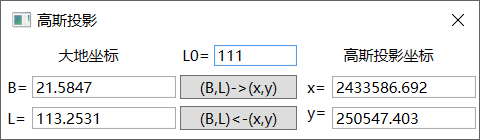
\includegraphics[scale=1]{gaussProj/UI01.png}
    \caption{简单的高斯投影正反算界面}
    \label{fig:GaussProjUI01}
\end{figure}

相应的主要界面代码如下:

\begin{lstlisting}[language=xml]
<TextBlock Text="大地坐标" HorizontalAlignment="Center"
        VerticalAlignment="Center"/>
<TextBlock  Text="B=" Grid.Row="1" Margin="5"/>
<TextBox x:Name="textBox_B" Grid.Row="1"
        Text=""
        VerticalAlignment="Center"  Margin="25,0,0,0"/>
<TextBlock  Text="L=" Margin="5" Grid.Row="2" />
<TextBox x:Name="textBox_L"
        Text=""
        VerticalAlignment="Center" Margin="25,0,0,0" Grid.Row="2" />

<TextBlock  Text="L0=" Grid.Column="1"
        Margin="5,0,0,0" VerticalAlignment="Center"/>
<TextBox x:Name="textBox_L0"
        Text=""
        Grid.Column="1"
        Margin="30,0,3,0" VerticalAlignment="Center"/>
<Button Content="(B,L)->(x,y)" Grid.Column="1" Grid.Row="1"
                Click="BLtoXYButton_Click" Margin="3,3"/>
<Button Content="(B,L)&lt;-(x,y)" Grid.Column="1" Grid.Row="2"
                Click="XYtoBLButton_Click"  Margin="3,3"/>
        
<TextBlock Text="高斯投影坐标" Grid.Column="2"
                HorizontalAlignment="Center" VerticalAlignment="Center"/>
<TextBlock  Text="x=" Margin="5" Grid.Row="1" Grid.Column="2"/>
<TextBox x:Name="textBox_x" Grid.Row="1" Grid.Column="2"
                Text=""
                Margin="25,0,0,0" VerticalAlignment="Center" />
<TextBlock Text="y=" Grid.Row="2" Grid.Column="2" Margin="5,0,0,0"/>
<TextBox x:Name="textBox_y"
                Text=""
                Grid.Row="2"  Grid.Column="2"
                Margin="25,0,0,0" VerticalAlignment="Center" />       
\end{lstlisting}

请注意,在这段xaml界面代码中,由于我们的算法需要与界面上的TextBox控件进行数据交换,
每个TextBox都需要命名(如上的每个TextBox控件都有一个 x:Name 属性)。

相应的正算与反算按钮响应事件代码如下:

\begin{lstlisting}[language=C]
private void BLtoXYButton_Click(object sender, RoutedEventArgs e)
{
    double B, L, L0, x, y;
    double.TryParse(this.textBox_B.Text, out B);
    double.TryParse(this.textBox_L.Text, out L);
    double.TryParse(this.textBox_L0.Text, out L0);

    Spheroid proj = Spheroid.CreateBeiJing1954();
    proj.BLtoXY(
        ZXY.SMath.DMS2RAD(B),
        ZXY.SMath.DMS2RAD(L),
        ZXY.SMath.DMS2RAD(L0),
        out x, out y);
    this.textBox_x.Text = x.ToString();
    this.textBox_y.Text = y.ToString();
}

private void XYtoBLButton_Click(object sender, RoutedEventArgs e)
{
    double B, L, L0, x, y;
    double.TryParse(this.textBox_x.Text, out x);
    double.TryParse(this.textBox_y.Text, out y);
    double.TryParse(this.textBox_L0.Text, out L0);

    Spheroid proj = Spheroid.CreateBeiJing1954();
    proj.XYtoBL(x, y,
        ZXY.SMath.DMS2RAD(L0),
        out B, out L);
    this.textBox_B.Text =ZXY.SMath.RAD2DMS(B).ToString();
    this.textBox_L.Text = ZXY.SMath.RAD2DMS(L).ToString();
}
\end{lstlisting}

在这个两个响应事件中,首先需要直接从界面上的TextBox控件中取值,
由于TextBox的Text属性是文本(string类型),需要用double.TryParse
函数将其转换为double类型。

其次我们默认参考椭球为1954北京坐标系的参考椭球,需要将其创建,此处我们用
类的静态函数可以方便创建,不必记忆其椭球的几何参数值。

然后我们就可以调用我们前边写的正算与反算函数进行高斯投影正反算了,算完后
将值再赋值给相应的TextBox控件的Text属性就可以了。注意传入函数的值如果是度分秒形式的角度,
应该先调用我们前边的写的函数将其转换为弧度,如果算出的值也是角度,也应该调用我们
前面所写的函数将其转换为度分秒形式。


\subsection{界面程序的优化}
上面的简单界面程序存在着一个很大的问题,就是从界面取数据时无法判断数据的有效性等,
也无法发挥WPF界面技术。WPF界面技术里的数据绑定功能(binding)可以很好的简化这一过程。

我们仔细分析前边的界面,这个程序的实质就是一个点的两种形式的坐标之间的转换,
因此我们可以定义一个点类GeoPoint,其定义如下:

\begin{lstlisting}[language=C]
public class GeoPoint
{
    public string Name { get; set;} //点名
    public double B { get; set;}    //纬度,单位:度分秒
    public double L { get; set;}    //经度,单位:度分秒
    public double L0 { get; set;}   //中央子午线经度,单位:度分秒
    public double X { get; set;}    //X坐标
    public double Y { get; set;}    //Y坐标
}
\end{lstlisting}

则在界面代码中可对TextBox的Text做如下绑定:

\begin{lstlisting}[language=C]
<TextBlock Text="大地坐标" HorizontalAlignment="Center"
        VerticalAlignment="Center"/>
<TextBlock  Text="B=" Grid.Row="1" Margin="5"/>
<TextBox x:Name="textBox_B" Grid.Row="1"
        Text="{Binding B}"
        VerticalAlignment="Center"  Margin="25,0,0,0"/>
<TextBlock  Text="L=" Margin="5" Grid.Row="2" />
<TextBox x:Name="textBox_L"
        Text="{Binding L}"
        VerticalAlignment="Center" Margin="25,0,0,0" Grid.Row="2" />

<TextBlock  Text="L0=" Grid.Column="1"
        Margin="5,0,0,0" VerticalAlignment="Center"/>
<TextBox x:Name="textBox_L0"
        Text="{Binding L0}" 
        Grid.Column="1"
        Margin="30,0,3,0" VerticalAlignment="Center"/>
<Button Content="(B,L)->(x,y)" Grid.Column="1" Grid.Row="1"
        Click="BLtoXYButton_Click" Margin="3,3"/>
<Button Content="(B,L)&lt;-(x,y)" Grid.Column="1" Grid.Row="2"
        Click="XYtoBLButton_Click"  Margin="3,3"/>
        
<TextBlock Text="高斯投影坐标" Grid.Column="2"
        HorizontalAlignment="Center" VerticalAlignment="Center"/>
<TextBlock  Text="x=" Margin="5" Grid.Row="1" Grid.Column="2"/>
<TextBox x:Name="textBox_x" Grid.Row="1" Grid.Column="2"
        Text="{Binding X}"
        Margin="25,0,0,0" VerticalAlignment="Center" />
<TextBlock Text="y=" Grid.Row="2" Grid.Column="2" Margin="5,0,0,0"/>
<TextBox x:Name="textBox_y"
        Text="{Binding Y}"
        Grid.Row="2"  Grid.Column="2"
        Margin="25,0,0,0" VerticalAlignment="Center" />  
\end{lstlisting}

以上代码中的TextBox控件中的x:Name属性甚至都可以省略。由于这些控件都是
以这个窗体(Window)作为容器的,他们的数据源都可用这个窗体的DataContext
一次性设置,让系统以冒泡的形式自动为属性绑定寻找数据源。窗体为之
设定数据源的代码如下:

\begin{lstlisting}[language=C]
public partial class MainWindow : Window
{
    private GeoPoint geoPoint;
    private Spheroid proj = Spheroid.CreateBeiJing1954();

    public MainWindow()
    {
        InitializeComponent();
        geoPoint = new GeoPoint(){ B= 21.58470845, L= 113.25314880 };
        this.DataContext = geoPoint;
    }
    //.......省略了其他代码......
}
\end{lstlisting}

程序中由于正反算都是基于相同的椭球基准,所以在类MainWindow中定义了
geoPoint实例字段与proj实例字段。在构造函数中为其赋了初值以简化每次在
界面输入数据,为这个窗体的DataContext指定点的各项属性绑定的数据源。

相应的正反算按钮的响应事件修改为:

\begin{lstlisting}[language=C]
private void BLtoXYButton_Click(object sender, RoutedEventArgs e)
{
    double x, y;
    proj.BLtoXY(
        ZXY.SMath.DMS2RAD(geoPoint.B),
        ZXY.SMath.DMS2RAD(geoPoint.L),
        ZXY.SMath.DMS2RAD(geoPoint.L0),
        out x, out y);
    geoPoint.X = x; geoPoint.Y = y;
}

private void XYtoBLButton_Click(object sender, RoutedEventArgs e)
{
    double B, L;
    proj.XYtoBL(geoPoint.X, geoPoint.Y,
       ZXY.SMath.DMS2RAD(geoPoint.L0),
       out B, out L);
    geoPoint.B = ZXY.SMath.RAD2DMS(B);
    geoPoint.L = ZXY.SMath.RAD2DMS(L);
}
\end{lstlisting}

从响应事件可以看出,代码简洁了很多。运行程序时,TextBox框中都有默认数值,
而且非数值数据也输入不进去了,也不需要将文本框中的Text属性转换为double类型了。
一切看似都好,但你发现在点击正算或反算按钮时,界面上的数据没有变化,好像功能没有实现一样,
问题出现在什么地方呢?

我们回过头再看GeoPoint的定义,发现其属性定义过于简单。根据WPF知识可知,在对象属性发生改变时
(如我们的计算中正算改变了X与Y,反算改变了B与L),还需要一种机制通知系统需要刷新界面,
这就需要类GeoPoint从接口 INotifyPropertyChanged 继承并实现它
(该接口所在的命名空间为System.ComponentModel)。修改后的GeoPoint类如下:

\begin{lstlisting}[language=C]
public class GeoPoint : INotifyPropertyChanged
{
    public event PropertyChangedEventHandler PropertyChanged;

    public void RaisePropertyChange(string propertyName)
    {
        if (this.PropertyChanged != null)
        {
            this.PropertyChanged.Invoke(this, 
                new PropertyChangedEventArgs(propertyName));
        }
    }

    private string _name;
    public string Name //点名
    {
        get { return _name; }
        set
        {
            _name = value;
            RaisePropertyChange("Name");
        }
    }

    private double _B;
    public double B //纬度,单位:度分秒
    {
        get { return _B; }
        set
        {
            _B = value;
            RaisePropertyChange("B");
        }
    }

    private double _L;
    public double L //经度,单位:度分秒
    {
        get { return _L; }
        set
        {
            _L = value;
            RaisePropertyChange("L");
        }
    }

    private double _L0;
    public double L0 //中央子午线经度,单位:度分秒
    {
        get { return _L0; }
        set
        {
            _L0 = value;
            RaisePropertyChange("L0");
        }
    }

    private double _X;
    public double X //X坐标
    {
        get { return _X; }
        set
        {
            _X = value;
            RaisePropertyChange("X");
        }
    }
  
    private double _Y;
    public double Y  //Y坐标
    {
        get { return _Y; }
        set
        {
            _Y = value;
            RaisePropertyChange("Y");
        }
    }
}
\end{lstlisting}

与前面的GeoPoint类相比较,现在的这个类从 INotifyPropertyChanged 继承
并实现了接口成员PropertyChanged,在属性值发生改变时利用该接口成员通知界面
属性值发生了变化。

运行程序,功能一切正常。


\subsection{点类的进一步优化}

我们再次审阅界面程序后的正反算代码,发现事实上的正反算都是基于点类的,
也就是说只与GeoPoint类相关,因此我们将正反算功能移到GeoPoint类中,
以进一步简化界面的方法调用。其代码如下:

\begin{lstlisting}[language=C]
public class GeoPoint : INotifyPropertyChanged
{
    //......其它代码.......
    public void BLtoXY(Spheroid spheroid)
    {
        double x, y;
        spheroid.BLtoXY(
           ZXY.SMath.DMS2RAD(this.B),
           ZXY.SMath.DMS2RAD(this.L),
           ZXY.SMath.DMS2RAD(this.L0),
           out x, out y);
        this.X = x; this.Y = y;
    }

    public void XYtoBL(Spheroid spheroid)
    {
        double B, L;
        spheroid.XYtoBL(X, Y, ZXY.SMath.DMS2RAD(this.L0),
           out B, out L);
        this.B = ZXY.SMath.RAD2DMS(B);
        this.L = ZXY.SMath.RAD2DMS(L);
    }
}
\end{lstlisting}

界面正反算代码可以进一步简化为如下形式:

\begin{lstlisting}[language=C]
private void BLtoXYButton_Click(object sender, RoutedEventArgs e)
{
    geoPoint.BLtoXY(proj);
}

private void XYtoBLButton_Click(object sender, RoutedEventArgs e)
{
    geoPoint.XYtoBL(proj) ;
}
\end{lstlisting}

至此,我们的算法与界面几乎是完全分离了,这符合我们第一章所讲的界面与算法相
分离的原则,也为我们的算法进行单元测试和进一步优化迭代打下了基础。


\section{更加实用的多点计算图形程序}

上面的程序从编程的角度讲比较完美了,但从实用的角度来说还有很多缺点,
比如不能选择椭球基准,不能进行多点的正反算,不能读取和写出文本文件数据。
这一节我们将从算法和界面两个方面来构造这个更加实用的多点高斯投影计算的
图形程序。

\subsection{程序的功能}

实用的高斯投影程序功能如下:

\begin{enumerate}
\item 椭球基准的选择:能够自由的选择参考椭球基准,或者自定义参考椭球;
\item 能实现高斯投影正反算与换带功能;
\item 高斯投影坐标的定义:能自动去除或添加点的Y坐标前的常数500km和带号;
\item 数据的界面录入:能利用程序界面组织输入数据;
\item 能导入导出文本数据:能将外部文本数据导入到程序中,能将程序中的数据导出为文本文件;
\item 能实现多个点的批量计算。
\end{enumerate}

软件运行时的界面如图\ref{fig:GaussProjUI02}所示,该界面基本能满足以上功能。

\begin{figure}[htbp]
    \centering
    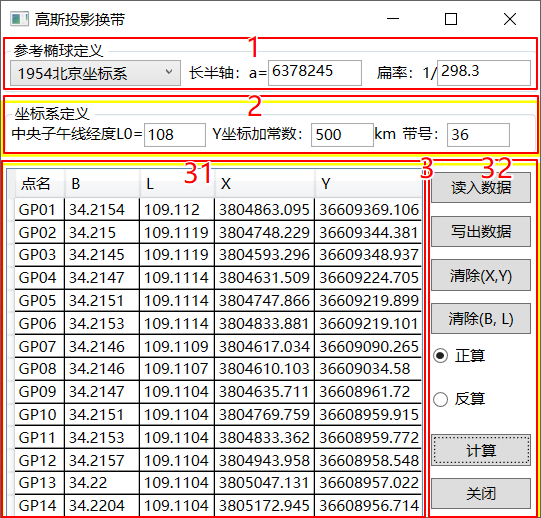
\includegraphics[scale=1]{gaussProj/UI02.png}
    \caption{实用高斯投影程序界面}
    \label{fig:GaussProjUI02}
\end{figure}

\subsection{程序的面向对象分析与实现}

从界面上我们可以看出,程序中应该包含三部分内容:
椭球基准、坐标系、点集。为了满足以上功能,我们需要对我们的程序进行重构。

分析我们前边的 GeoPoint 类会发现,一个点有中央子午线经度 L0 这个属性会很奇怪,
而在实际应用中点集也是基于坐标系的点集,一个点集的y坐标甚至x坐标前的加常数也是基本相同。
因此坐标系应该有中央子午线经度 L0属性,带号N与Y坐标前的加常数YKM,
由于坐标系是依赖于椭球基准的,也应有椭球基准属性ProjSpheroid。
坐标系类的定义如下代码所示:

\begin{lstlisting}[language=C]
using System.Collections.ObjectModel;

/// <summary>
/// 坐标系
/// </summary>
public class CoordinateSystem : INotifyPropertyChanged
{
    //....省略与接口INotifyPropertyChanged有关的代码....

    /// <summary>
    /// 中央子午线经度
    /// </summary>
    private double _L0;
    
    /// <summary>
    /// 中央子午线经度
    /// </summary>
    public double L0
    {
        get { return _L0; }
        set
        {
            _L0 = value;
            RaisePropertyChange("L0");
        }
    }
    
    /// <summary>
    /// 带号
    /// </summary>
    private int _N;
    
    /// <summary>
    /// 带号
    /// </summary>
    public int N
    {
        get { return _N; }
        set
        {
            _N = value;
            RaisePropertyChange("N");
        }
    }
    
    /// <summary>
    /// Y坐标的加常数
    /// </summary>
    private double _YKM;
    
    /// <summary>
    /// Y坐标的加常数
    /// </summary>
    public double YKM
    {
        get { return _YKM; }
        set
        {
            _YKM = value;
            RaisePropertyChange("YKM");
        }
    }
    
    /// <summary>
    /// 坐标点集
    /// </summary>
    private ObservableCollection<GeoPoint>geoPointList = 
        new ObservableCollection<GeoPoint>();
    
    /// <summary>
    /// 坐标点集
    /// </summary>
    public ObservableCollection<GeoPoint> GeoPointList
    {
        get { return geoPointList; }
    }
    
    /// <summary>
    /// 投影椭球基准
    /// </summary>
    private Spheroid spheroid = Spheroid.CreateBeiJing1954();
    
    /// <summary>
    /// 投影椭球基准
    /// </summary>
    public Spheroid ProjSpheroid
    {
        get { return spheroid; }
        set
        {
            spheroid = value;
            RaisePropertyChange("ProjSpheroid");
        }
    }

   public CoordinateSystem(){ }
}
\end{lstlisting}

在类GeoPoint中将属性L0的定义删除。在CoordinateSystem类中,由于
N,L0,YKM需与界面交互,故须从接口 INotifyPropertyChanged 继承。

为与WPF界面中的DataGrid控件交互,点集需要用ObservableCollection<GPoint> 表达,
不能用List<GPoint>,而且默认状态下就应该生成其实例对象。注意二者的命名空间也不一样,
前者为System.Collections.ObjectModel,
用于界面交互较多,后者为 System.Collections.Generic,用于不需要界面的
算法较多。

为了与界面的初始状态一致,对投影的参考椭球我们默认生成北京54坐标系的
参考椭球。

在我们的程序中GeoPoint类与CoordinateSystem类为了处理与界面交互的
问题,都需要实现接口 INotifyPropertyChanged,实现接口的代码重复。
本着相同或相似的代码在程序中只写一次的原则,我们将这部分的代码独立到
类 NotificationObject 中,让GeoPoint类与CoordinateSystem类从
NotificationObject 类继承。相应的实现代码如下:

\begin{lstlisting}[language=C]
using System.ComponentModel;

namespace GaussProj
{
    public class NotificationObject : INotifyPropertyChanged
    {
        public event PropertyChangedEventHandler PropertyChanged;

        public void RaisePropertyChange(string propertyName)
        {
            if (this.PropertyChanged != null)
            {
                this.PropertyChanged.Invoke(this, new PropertyChangedEventArgs(propertyName));
            }
        }
    }
}

public class GeoPoint : NotificationObject
{
    //删除与NotificationObject类中相同的代码
    //省略GeoPoint类中的内容
}

public class CoordinateSystem : NotificationObject
{
    //删除与NotificationObject类中相同的代码
    //省略CoordinateSystem类中的内容
}
\end{lstlisting}

\subsection{多点的高斯投影计算}

如此,在类CoordinateSystem中就有了用于高斯投影的椭球基准,
有了坐标系的中央子午线经度,有了带号及y坐标前的加常数与点集,
多点的高斯投影计算就万事俱备,只欠实现了。其实现代码如下:

\begin{lstlisting}[language=C]
public class CoordinateSystem : NotificationObject 
{
    //省略其他代码

    /// <summary>
    /// 多点高斯投影正算
    /// </summary>
    public void BLtoXY()
    {
        foreach (var pnt in this.geoPointList)
        {
            pnt.BLtoXY(spheroid, this);
        }
    }

    /// <summary>
    /// 多点高斯投影反算
    /// </summary>
    public void XYtoBL()
    {
        foreach (var pnt in this.geoPointList)
        {
            pnt.XYtoBL(spheroid, this);
        }
    }
}
\end{lstlisting}

从代码中可以看出,在类CoordinateSystem中并没有真正的进行高斯投影正算与
反算,而是通过循环将其委托给每个点的实例了。

点类GeoPoint中的高斯投影正反算实现如下:

\begin{lstlisting}[language=C]
public class GeoPoint : NotificationObject
{
    //省略其他代码
    /// <summary>
    /// 高斯投影正算
    /// </summary>
    /// <param name="spheroid">投影椭球</param>
    /// <param name="cs">坐标系</param>
    public void BLtoXY(Spheroid spheroid, CoordinateSystem cs)
    {
        double x, y;
        spheroid.BLtoXY(
           ZXY.SMath.DMS2RAD(this.B),
           ZXY.SMath.DMS2RAD(this.L),
           ZXY.SMath.DMS2RAD(cs.L0),
           out x, out y);
        this.X = x; this.Y = y + cs.YKM * 1000 + cs.N * 1000000;
    }
    /// <summary>
    /// 高斯投影反算
    /// </summary>
    /// <param name="spheroid">投影椭球</param>
    /// <param name="cs">坐标系</param>
    public void XYtoBL(Spheroid spheroid, CoordinateSystem cs)
    {
        double tB, tL;
        double y = Y - cs.YKM * 1000 - cs.N * 1000000;
        spheroid.XYtoBL(X, y, ZXY.SMath.DMS2RAD(cs.L0),
           out tB, out tL);
        this.B = ZXY.SMath.RAD2DMS(tB);
        this.L = ZXY.SMath.RAD2DMS(tL);
    }
}
\end{lstlisting}

从如上的代码中可以看出,真正的高斯投影正反算还是在我们前面写的Spheroid类中。
请注意在Spheroid类中,所有的与角度有关的单位是弧度,y坐标也是点的真实坐标,
在此我们需要根据坐标系中的信息对其做相应的预处理。

还应注意,在BLtoXY中,为了与界面交互,要赋值给this.X与this.Y,而不是赋值给其变量
this.\_X与this.\_Y。在 XYtoBL 中也同样如此,当然还需要将计算出的弧度值转换为度分秒形式。

\subsection{点坐标数据的读入与写出}

利用我们的界面可以手工输入点的坐标数据,但导入与导出文本数据对于一个
程序来讲是必不可少的功能。

为了避免我们的教学程序过于复杂,我们对数据文件的格式进行适当简化。

在高斯投影正算时,所需的数据应该是:点名,纬度B, 经度L,设计我们的文本文件
内容如下:

\begin{verbatim}
 #点名,   B,   L
GP01,34.2154,109.112
GP02,34.215,109.1119
GP03,34.2145,109.1119
GP04,34.2147,109.1114
GP05,34.2151,109.1114
\end{verbatim}

文件中的每一行第一个字符以 \#开头的我们视为注释行,予以忽略。

在高斯投影反算时,所需的数据应该是:点名,X, Y,设计我们的文本文件
内容如下:

\begin{verbatim}
#点名,       X,       Y,         H
GP01, 3805709.2106, 19333388.3123, 466.419
GP02, 3805595.1034, 19333360.1973, 470.94
GP03, 3805440.0738, 19333360.1727, 478.728
GP04, 3805481.9494, 19333237.0999, 475.975
GP05, 3805598.4201, 19333235.7343, 469.738
\end{verbatim}

文件中的数据项可以多余三项,我们只读取第1、2、3项,其余忽略。

在写出数据时,我们将点的五项数据:点名,B, L, X, Y 全部写出,
如下所示:

\begin{verbatim}
# 点名,    B,      L,     X,      Y 
GP01, 34.2154, 109.112  , 3804863.095, 36609369.106
GP02, 34.215,   109.1119, 3804748.229, 36609344.381
GP03, 34.2145, 109.1119, 3804593.296, 36609348.937
GP04, 34.2147, 109.1114, 3804631.509, 36609224.705
GP05, 34.2151, 109.1114, 3804747.866, 36609219.899
\end{verbatim}

用户在使用时可以将其数据拷贝到Word中按分隔符 ``,''生成表格进行编辑
处理,或按分隔符 ``,''导入到Excel中进行编辑排版处理。

读入的点坐标数据应存储在我们的程序中,很显然应该在类CoordinateSystem中
实现读入文本文件数据功能,写出数据的功能也如此,其实现代码如下:

\begin{lstlisting}[language=C]
public class CoordinateSystem : NotificationObject 
{
    //省略其他代码

    /// <summary>
    /// 读入点集坐标数据
    /// </summary>
    /// <param name="fileName">文件名</param>
    /// <param name="format">点的坐标格式:BL-Name,B,L  
    ///                                 XY-Name,X,Y
    /// </param>
    public void ReadGeoPointData(string fileName, string format)
    {
        using (System.IO.StreamReader sr = new System.IO.StreamReader(fileName) )
        {
            string buffer;
            //读入点的坐标数据
            this.GeoPointList.Clear();
            while (true)
            {
                buffer = sr.ReadLine();
                if (string.IsNullOrEmpty(buffer)) break; //文件末尾或空行退出
                if (buffer[0] == '#') continue;
                string[] its = buffer.Split(new char[1] { ',' });
                if (its.Length < 3) continue; //少于三项数据,不是点的坐标数据,忽略
                GeoPoint pnt = new GeoPoint();
                pnt.Name = its[0].Trim(); 
                if (format == "XY")
                {                       
                    pnt.X = double.Parse(its[1]); 
                    pnt.Y = double.Parse(its[2]);
                    pnt.B = 0; pnt.L = 0;
                }
                else if (format == "BL")
                {
                    pnt.B = double.Parse(its[1]); 
                    pnt.L = double.Parse(its[2]); 
                    pnt.X = 0; pnt.Y = 0;
                }
               
                this.GeoPointList.Add(pnt);
            }
        }
    }

    /// <summary>
    /// 写出点集坐标数据
    /// </summary>
    /// <param name="fileName">文件名</param>
    public void WriteGeoPointData(string fileName)
    {
        using (System.IO.StreamWriter sr = new System.IO.StreamWriter(fileName))
        {
            sr.WriteLine("#点名,   B,   L,  X,  Y");
            foreach (var pnt in this.geoPointList)
            {
                sr.WriteLine( pnt );
            }
        }
    }
}
\end{lstlisting}

写数据比较简单,按要求写出即可,需要注意的是第57行,在函数WriteLine中
我们直接写出了GeoPoint的实例对象pnt,这需要在GeoPoint中将ToString()
进行override,实现代码如下:
\begin{lstlisting}[language=C]
public class GeoPoint : NotificationObject
{
    public override string ToString()
    {
        return string.Format("{0},{1:0.0000},{2:0.0000},{3:0.000},{4:0.000}", Name, B, L, X, Y);
    }
}
\end{lstlisting}

在占位符中我们加入了输出浮点数据的格式控制,保证输出的角度小数位数不超过四位,
输出的坐标不超过三位。

读入数据相对于写出数据要由于需要解码数据,所以要复杂一些。小于三个数据项
的行我们直接略过,同时我们能加入格式控制,如果格式控制BL,
意味着数据文件是经纬度数据,其他属性相应置零。

读入数据的这段代码我们实现的方式较为粗略,只是通过逗号分隔的数据项个数
进行了判断,这在真正的程序开发中是不可靠的,可以通过正则表达式对每行数据进行检验,
对符合要求的文本数据加以处理,以此来提高读取文本数据功能的容错能力。

清除(X, Y)与清除(B, L)功能实质上是将点的这些属性置零,比较简单,相应代码如下:

\begin{lstlisting}[language=C]
public class CoordinateSystem : NotificationObject 
{
    //省略其他代码

    public void ClearXY()
    {
        foreach (var pnt in this.geoPointList)
        {
            pnt.X = pnt.Y = 0;
        }
    }
    public void ClearBL()
    {
        foreach (var pnt in this.geoPointList)
        {
            pnt.B = pnt.L = 0;
        }
    }
}
\end{lstlisting}


\subsection{界面设计与实现}

按图\ref{fig:GaussProjUI02}设计的界面代码如下:

\begin{lstlisting}[language=xml]
<Window x:Class="GaussProj.GaussProjWin"
        xmlns="http://schemas.microsoft.com/winfx/2006/xaml/presentation"
        xmlns:x="http://schemas.microsoft.com/winfx/2006/xaml"
        xmlns:d="http://schemas.microsoft.com/expression/blend/2008"
        xmlns:mc="http://schemas.openxmlformats.org/markup-compatibility/2006"
        xmlns:local="clr-namespace:GaussProj"
        mc:Ignorable="d"
        Title="高斯投影换带" Height="360" Width="540">
    <Grid>
        <Grid.RowDefinitions>
            <RowDefinition Height="45"/>
            <RowDefinition Height="5"/>
            <RowDefinition Height="45"/>
            <RowDefinition Height="5"/>
            <RowDefinition Height="Auto"/>
        </Grid.RowDefinitions>
        <GroupBox x:Name="groupBox_spheroid" Header="参考椭球定义" 
            DataContext="ProjSpheroid" Margin="1">
            <Grid>
                <Grid.ColumnDefinitions>
                    <ColumnDefinition Width="200*"/>
                    <ColumnDefinition Width="70"/>
                    <ColumnDefinition Width="110*"/>
                    <ColumnDefinition Width="60"/>
                    <ColumnDefinition Width="110*"/>
                </Grid.ColumnDefinitions>
                <ComboBox Grid.Column="0" x:Name="comboBox_Spheroid" 
                          SelectionChanged="comboBox_Spheroid_SelectionChanged">
                    <ComboBoxItem  Content="1954北京坐标系" Tag="BJ1954"/>
                    <ComboBoxItem Content="1980西安坐标系" Tag="XA1980"/>
                    <ComboBoxItem Content="CGCS2000大地坐标系" Tag="CGCS2000"/>
                    <ComboBoxItem Content="自定义参考椭球" Tag="CS0000"/>
                </ComboBox>
                <TextBlock Text="长半轴:a=" Grid.Column="1" 
                    VerticalAlignment="Center" HorizontalAlignment="Right"/>
                <TextBox x:Name="textBox_a" Grid.Column="2" Text="{Binding a}"/>
                <TextBlock Text="扁率:1/" Grid.Column="3" 
                    VerticalAlignment="Center" HorizontalAlignment="Right"/>
                <TextBox x:Name="textBox_f" Grid.Column="4" Text="{Binding f}"/>
            </Grid>
        </GroupBox>

        <Border  Grid.Row="2" BorderBrush="Yellow" BorderThickness="2">
            <GroupBox x:Name="groupBox_CoordinateSystem" Header="坐标系定义">
            <StackPanel Orientation="Horizontal">
                <TextBlock Text="中央子午线经度L0=" />
                <TextBox x:Name="textBox_L0" Text="{Binding L0}" Width="50"/>
                <TextBlock Text="Y坐标加常数:" Margin="5,0,0,0" />
                <TextBox x:Name="textBox_YKM" Text="{Binding YKM}" Width="50"/>
                <TextBlock Text="km" />
                <TextBlock Text="带号:" Margin="5,0,0,0"/>
                <TextBox x:Name="textBox_N" Text="{Binding N}" Width="50"/>
            </StackPanel>
            </GroupBox>
        </Border>
        
        <Border  Grid.Row="4" BorderBrush="Yellow" BorderThickness="2">
            <Grid>
                <Grid.ColumnDefinitions>
                    <ColumnDefinition Width="200*"/>
                    <ColumnDefinition Width="90"/>
                </Grid.ColumnDefinitions>
                <DataGrid x:Name="dataGrid_ctrPnt" 
                    AutoGenerateColumns="False" Margin="2" 
                    ItemsSource="{Binding GeoPointList}" >
                <DataGrid.Columns>
                    <DataGridTextColumn Header="点名" 
                        Binding="{Binding Name}"
                        MinWidth="40"/>
                    <DataGridTextColumn Header="B" 
                        Binding="{Binding B , StringFormat={}{0:##0.####}}" 
                        MinWidth="60"/>
                    <DataGridTextColumn Header="L" 
                        Binding="{Binding L , StringFormat={}{0:##0.####}}" 
                        MinWidth="60"/>
                    <DataGridTextColumn Header="X" 
                        Binding="{Binding X , StringFormat={}{0:##0.###}}" 
                        MinWidth="60"/>
                    <DataGridTextColumn Header="Y" 
                        Binding="{Binding Y, StringFormat={}{0:##0.###}}"
                        MinWidth="60" />
                </DataGrid.Columns>
            </DataGrid>

                <StackPanel Grid.Column="1" Orientation="Vertical">
                    <RadioButton x:Name="radioButton_BLtoXY"  Content="正算" 
                        Height="25" Width="80" Margin="5"/>
                    <RadioButton x:Name="radioButton_XYtoBL"  Content="反算" 
                        IsChecked="True" Height="25" Width="80" Margin="5" />

                    <Button x:Name="Button_ReadGaussProjData" Content="读入数据"
                        Height="25" Width="80" Margin="5" 
                        Click="Button_ReadGaussProjData_Click"/>
                    <Button x:Name="Button_WriteGaussProjData" Content="写出数据" 
                        Height="25" Width="80" Margin="5" 
                        Click="Button_WriteGaussProjData_Click"/>

                    <Button x:Name="Button_ClearXY" Content="清除(X,Y)" 
                        Height="25" Width="80" Margin="5" 
                        Click="Button_ClearXY_Click"/>
                    <Button x:Name="Button_ClearBL" Content="清除(B, L)" 
                        Height="25" Width="80" Margin="5" 
                        Click="Button_ClearBL_Click"/>
                    
                    <Button x:Name="Button_CalGaussProj"  Content="计算" 
                        Height="25" Width="80" Margin="5" 
                        Click="Button_CalGaussProj_Click"/>
                    <Button x:Name="Button_Close" Content="关闭" 
                        Height="25" Width="80" Margin="5" 
                        Click="Button_Close_Click"/>
                </StackPanel>
            </Grid>
        </Border>     
    </Grid>
</Window>
\end{lstlisting}

在这段xaml代码中,除了功能按钮区外,实际上分为了三部分:

第一部分为参考椭球定义,如第18行代码所示,我们将其布局到
 groupBox\_spheroid中,数据绑定a与f,数据源设置在groupBox\_spheroid中,
 采用冒泡搜寻类CoordinateSystem中的ProjSpheroid属性。

为了简化示例程序的编写,ComboBox中的参考椭球类型采用硬编码方式直接写在其中了。
通过SelectionChange事件对不同的椭球类型选择进行响应。

第二部分为坐标系定义,同样采用数据绑定的形式与界面交互数据,数据源来自
类CoordinateSystem。

第三部分为点集部分,数据源为类CoordinateSystem中的GeoPointList属性,如
第65行代码所示。

界面后台代码如下:

\begin{lstlisting}[language=C]
public partial class GaussProjWin : Window
{       
    private CoordinateSystem myCoordinateSystem;

    public GaussProjWin()
    {
        InitializeComponent();

        myCoordinateSystem = new CoordinateSystem() {
            L0 = 111, N = 19, YKM = 500};
        this.DataContext = myCoordinateSystem;

        this.comboBox_Spheroid.SelectedIndex = 0;
    }

    //省略其他代码
}
\end{lstlisting}

在窗体后台代码中,我们设置了窗体类的类实例变量myCoordinateSystem完成
各项功能。在其窗体类的构造函数中实例化并对其属性赋了初始值,同时将
窗体的DataContex属性设为myCoordinateSystem,完成数据绑定的数据源设置。
同时为了维持与界面属性的一致性,将comboBox\_Spheroid的SelectedIndex设为0。

界面的其它功能按钮的实现比较简单,实现代码如下:

\begin{lstlisting}[language=C]
public partial class GaussProjWin : Window
{   
    //省略其他代码

    private void comboBox_Spheroid_SelectionChanged(object sender, 
        SelectionChangedEventArgs e)
    {
        if(comboBox_Spheroid.SelectedIndex == 0)
            myCoordinateSystem.ProjSpheroid = Spheroid.CreateBeiJing1954();
        else if (comboBox_Spheroid.SelectedIndex == 1)
            myCoordinateSystem.ProjSpheroid = Spheroid.CreateXian1980();
        else if (comboBox_Spheroid.SelectedIndex == 2)
            myCoordinateSystem.ProjSpheroid = Spheroid.CreateCGCS2000();
        else if (comboBox_Spheroid.SelectedIndex == 3)
            myCoordinateSystem.ProjSpheroid = 
                Spheroid.CreateCoordinateSystem(6378137, 298.257222101);
        this.groupBox_spheroid.DataContext = myCoordinateSystem.ProjSpheroid;
    }

    private void Button_ReadGaussProjData_Click(object sender,
        RoutedEventArgs e)
    {
        OpenFileDialog dlg = new OpenFileDialog();
        dlg.DefaultExt = ".txt";
        dlg.Filter = "高斯投影坐标数据|*.txt|All File(*.*)|*.*";
        if (dlg.ShowDialog() != true) return;

        if (this.radioButton_BLtoXY.IsChecked == true)
            myCoordinateSystem.ReadGeoPointData(dlg.FileName, "BL");
        else if(this.radioButton_XYtoBL.IsChecked == true)
            myCoordinateSystem.ReadGeoPointData(dlg.FileName, "XY");
    }

    private void Button_WriteGaussProjData_Click(object sender, 
        RoutedEventArgs e)
    {
        SaveFileDialog dlg = new SaveFileDialog();
        dlg.DefaultExt = ".txt";
        dlg.Filter = "高斯投影坐标数据|*.txt|All File(*.*)|*.*";
        if (dlg.ShowDialog() != true) return;

        myCoordinateSystem.WriteGeoPointData(dlg.FileName);
    }

    private void Button_ClearXY_Click(object sender, RoutedEventArgs e)
    {
        myCoordinateSystem.ClearXY();
    }

    private void Button_ClearBL_Click(object sender, RoutedEventArgs e)
    {
        myCoordinateSystem.ClearBL();
    }

    private void Button_CalGaussProj_Click(object sender, RoutedEventArgs e)
    {
        if (radioButton_BLtoXY.IsChecked == true)
            myCoordinateSystem.BLtoXY();
        else if (radioButton_XYtoBL.IsChecked == true)
            myCoordinateSystem.XYtoBL();
    }

    private void Button_Close_Click(object sender, RoutedEventArgs e)
    {
        this.Close();
    }
}
\end{lstlisting}

\subsection{换带功能的实现}

在我们以上的设计中好像没有换带计算,虽然没有直接实现,但确实是实现了。
在前边的论述中,我们讲过,换带计算的实质是变换坐标系的中央子午线位置,
过程为:先进行坐标反算,然后变换中央子午线经度,再反算新的坐标即可。

\begin{figure}[htbp]
    \centering
    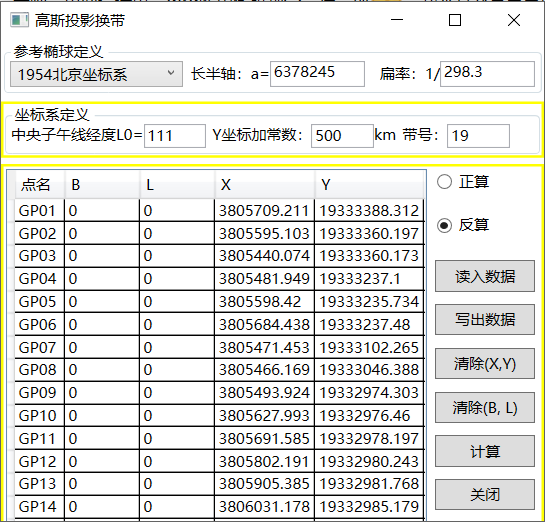
\includegraphics[scale=0.8]{gaussProj/UI03.png}
    \caption{$6\degree$带第19带数据界面}
    \label{fig:GaussProjUI03}
\end{figure}

启动程序,在反算的模式下读入数据,如图\ref{fig:GaussProjUI03}所示,这是一6度带第
19带的北京54坐标:

点击计算,反算各点的大地坐标经纬度,如图\ref{fig:GaussProjUI04}所示。

\begin{figure}[htbp]
    \centering
    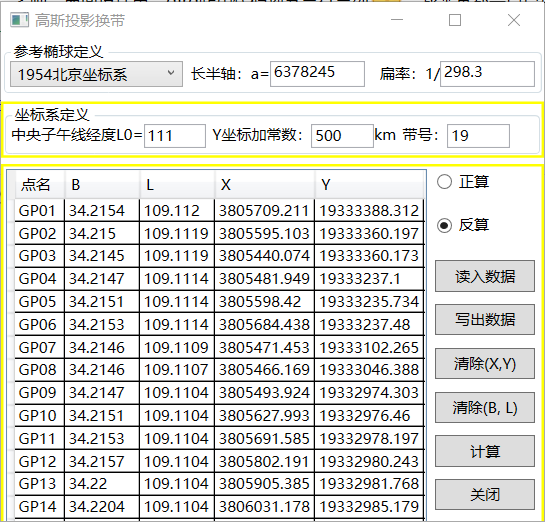
\includegraphics[scale=0.8]{gaussProj/UI04.png}
    \caption{$6\degree$带第19带反算数据界面}
    \label{fig:GaussProjUI04}
\end{figure}

现在我们准备将其换带到3度带的38带坐标系去,设置中央子午线经度L0为108,
带号设为36,选择正算,点击清除(x,y)按钮将X,Y坐标设置为0,如图\ref{fig:GaussProjUI05}所示:

\begin{figure}[htbp]
    \centering
    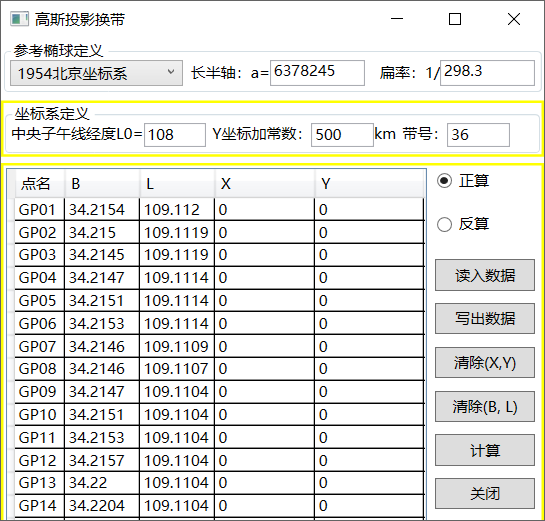
\includegraphics[scale=0.8]{gaussProj/UI05.png}
    \caption{设置$3\degree$带第36带数据界面}
    \label{fig:GaussProjUI05}
\end{figure}

点击计算按钮,计算出新坐标系下各点的坐标,如图\ref{fig:GaussProjUI06}所示:
\begin{figure}[htbp]
    \centering
    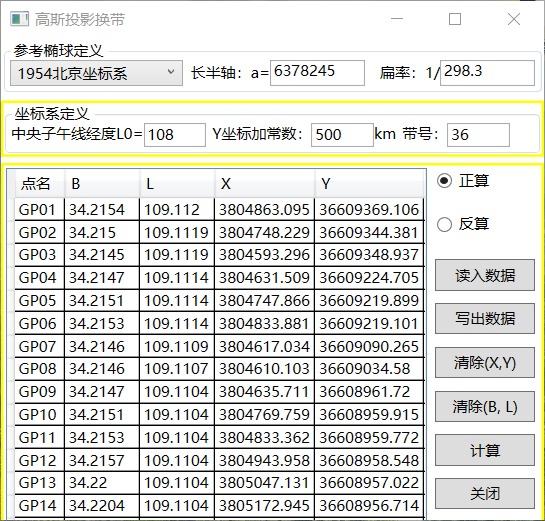
\includegraphics[scale=0.8]{gaussProj/UI06.png}
    \caption{$3\degree$带第36带正算数据界面}
    \label{fig:GaussProjUI06}
\end{figure}

到此就完成了换带功能,可以点击写出数据按钮将计算成果输出。

\section{UTM投影}

北半球: $x = x_r + 0$

南半球: $x = x_r + 10,000,000$, 加一万公里

Y坐标: $y = y_r + 500,000$, 加五百公里

需要注意的是:

UTM投影的分带与国际1:100万地图的划分一致,从 $180\degree$起向东每$6\degree$为一带。
因此, 高斯-克吕格投影的第一带($0\degree - 6\degree E$)为UTM投影的第31带,
UTM投影的第一带($180\degree - 174\degree W$)为高斯-克吕格投影的第31带.

\subsection{注意事项与功能扩展}

以上过程也可以看成是我们这个软件的教程。但应注意,换带计算只限于相同椭球
基准的情况才能应用,不能在不同椭球基准间应该该功能。

以上换带功能也可以设计一个界面,在新的界面上将新旧坐标系的中央子午线经度
都设置出,从而完成一键式换带计算功能。

我们经常在一些资料中见到椭球膨胀法建立独立坐标系或施工坐标系的方法,
椭球膨胀法是依据某种给定的参考椭球,根据测区的平均高程和平距纬度将
椭球面扩大而维持扁率不变,也可以应用换带的方法将椭球膨胀后的坐标与原坐标系的
坐标进行相互转换。但应注意椭球膨胀后,各个点的纬度值也会发生变化,
在这种换带过程中需要修正各个点的纬度值,大家可以参看这方面的资料。

随着我国对CGCS2000大地坐标系的推广应用与北斗导航系统的日益成熟,将大地坐标 $(B, L, H)$
与空间直角坐标 $(X, Y, Z)$ 进行相互转换的应用也会越来越多。如果能实现大地坐标 $(B, L, H)$
与空间直角坐标 $(X, Y, Z)$ 的相互转换,也就可以实现空间直角坐标 $(X, Y, Z)$
到高斯平面坐标的投影计算了,进而在桌面端电脑或移动设备上编程实现更多的功能应用。

大地坐标 $(B, L, H)$ 与空间直角坐标 $(X, Y, Z)$ 的相互转换公式如下:

已知大地坐标计算空间直角坐标的公式:
\begin{equation}
\left .
\begin{aligned}
X &= (N+H) \cos B \cos L \\
Y &= (N+H) \cos B \sin L \\
Z &= [N(1 - e^2) + H)] \sin B 
\end{aligned} 
\right \}
\end{equation}

已知空间直角坐标$(X,Y,Z)$计算大地坐标$(B, L, H)$的公式如下:

\begin{equation}
\left . 
\begin{aligned}
L &= \arctan \frac{Y}{X} \\
\tan B &= \frac{Z + Ne^2 \sin B}{\sqrt{X^2 + Y^2}} \\
H &= \frac{Z}{sinB} - N(1-e^2)  \\
 or  \\
H &=\frac{\sqrt{X^2 + Y^2}}{\cos B} - N 
\end{aligned} 
\right \}
\end{equation}

由以上公式可以看出,L可以直接有X,Y算出,B则需要迭代计算。

可对上面公式的B直接进行迭代计算,其过程如下:

% \begin{equation}
%     B = \arctan { \frac{Z+Ne^2 \sin B}{\sqrt{X^2 + Y^2}}}
% \end{equation}

先取B的初始值为:$B_0 =\arctan{ (Z / \sqrt{X^2 + Y^2} ) }$ 计算出$N$与$\sin B_0$,
代入上式,计算出新的B值$B_1$。然后将新的$B_1$代入再计算,直到两次的B值满足所要求的
精度。

或将:
$$N = \frac{c}{\sqrt{1+e'^2 \cos ^2 B}}$$
与$$\frac{1}{\cos^2 B} = 1+ \tan^2 B$$

代入到上式中,得到:
\begin{equation}
    \tan B = \frac{Z}{\sqrt{X^2 + Y^2}} + \frac{ce^2 \cdot \tan B}{\sqrt{X^2 + Y^2} \cdot \sqrt{1 + e'^2 + \tan^2 B}}
\end{equation}

则可令 $tB = \tan B$,对公式两边的 tB 进行迭代计算,当满足精度要求时,再求出B值$B=\arctan (tB)$即可。

本处只是列出了基本的计算公式与计算思路,大家可以查找资料寻找更加高效的计算方法予以实现。

\section*{小结}

我们从一个较为简单的单点高斯投影正反算程序开始,运用
C\#知识与WPF界面技术实现了一个较为实用的高斯投影正反算与换带
程序。

在程序过程中,我们遵循了界面与算法相分离的原则,运用了WPF的
事件绑定等技术。

这个程序从功能上讲还是有许多不足的,从易用性上也还有许多值得改进的
地方。希望随着我们的C\#知识与WPF技术的积累,能在以后将它优化得更好!
